%%%%%%%%%%%%%%%%%%%%%%%%%%%%%%%%%%%%%%%%%
% Dreuw & Deselaer's Poster
% LaTeX Template
% Version 1.0 (11/04/13)
%
% Created by:
% Philippe Dreuw and Thomas Deselaers
% http://www-i6.informatik.rwth-aachen.de/~dreuw/latexbeamerposter.php
%
% This template has been downloaded from:
% http://www.LaTeXTemplates.com
%
% Edited by: Fabian Kalweit und Manfred Brill
%
% License:
% CC BY-NC-SA 3.0 (http://creativecommons.org/licenses/by-nc-sa/3.0/)
%%%%%%%%%%%%%%%%%%%%%%%%%%%%%%%%%%%%%%%%%

% ----------------------------------------------------------------------------------------
%  Kopf- und Fusszeile werden in beamertheme16pd2.sty definiert!
% Diese Datei wurde so verändert, dass als Logo die Datei logo.png,
% mit dem Logo der Hochschule Kaiserslautern, verwendet wird!
% Auch die Fusszeile ist in dieser Datei definiert. Die dafür verwendeten
% Abbildungen liegen im Verzeichnis figures oder in Unterverzeichnissen.
%
% Dies entspricht der Vorlage für Poster im Projekt InfoStudi.
% ----------------------------------------------------------------------------------------

%----------------------------------------------------------------------------------------
%   PACKAGES AND OTHER DOCUMENT CONFIGURATIONS
%----------------------------------------------------------------------------------------
\documentclass[final,hyperref={pdfpagelabels=false}]{beamer}

\usepackage{todo}

\usepackage{wrapfig}

\usepackage[orientation=portrait,size=a0,scale=1.4]{beamerposter} % Use the beamerposter package for laying out the poster with a portrait orientation and an a0 paper size

% Use the I6pd2 theme supplied with this template
\usetheme{I6pd2} 

\usepackage[german]{babel}
%\usepackage[english]{babel} % English language/hyphenation

\usepackage{amsmath,amsthm,amssymb,latexsym} % For including math equations, theorems, symbols, etc

%\usepackage{times}\usefonttheme{professionalfonts}  % Uncomment to use Times as the main font
%\usefonttheme[onlymath]{serif} % Uncomment to use a Serif font within math environments

\boldmath % Use bold for everything within the math environment

\usepackage{booktabs} % Top and bottom rules for tables

\usepackage{multicol}


% Pfad für Abbildungen
\graphicspath{{figures/}} % Location of the graphics files

\usecaptiontemplate{\small\structure{\insertcaptionname~\insertcaptionnumber: }\insertcaption} % A fix for figure numbering

%----------------------------------------------------------------------------------------
%   TITLE SECTION
%----------------------------------------------------------------------------------------

\title{\huge Informatik studieren in der digitalen Gesellschaft} % Poster title

\author{Manfred Brill, Miriam Lohmüller, Pascal Pries} % Author(s)

\institute{Hochschule Kaiserslautern Fachbereich Informatik und Mikrosystemtechnik} % Institution(s)

%----------------------------------------------------------------------------------------
%   FOOTER TEXT
%----------------------------------------------------------------------------------------
%
\newcommand{\rightfoot}{manfred.brill@hs-kl.de} % Right footer text

%----------------------------------------------------------------------------------------

\begin{document}

\addtobeamertemplate{block end}{}{\vspace*{2ex}} % White space under blocks

\begin{frame}[t] % The whole poster is enclosed in one beamer frame

\begin{columns}[t] % The whole poster consists of two major columns, each of which can be subdivided further with another \begin{columns} block - the [t] argument aligns each column's content to the top

\begin{column}{.02\textwidth}\end{column} % Empty spacer column

\begin{column}{.465\textwidth} % The first column

%----------------------------------------------------------------------------------------
%   Peerleaders
%----------------------------------------------------------------------------------------

\begin{block}{Peerleaders}

    \vspace{40px}

    \begin{figure}
        \includegraphics[width=0.4\linewidth]{imagesExample/Peerleaders_Logo}
    \end{figure}

    \begin{itemize}
        \item Herausbildung interpersonaler Kompetenzen durch Peer-Gruppen
        \item Erh"ohung des Studienerfolgs durch gruppendynamische Prozesse
        \item Netzwerkbildung und  "Ubernahme von Verantwortung
        \item F"orderung der Empathief"ahigkeit
    \end{itemize}

        \vspace{20px}
    \begin{figure}
        \includegraphics[width=0.9\linewidth]{imagesExample/schaubild}
%       \caption{Schaubild}
    \end{figure}
    \vspace{40px}


\end{block}

%----------------------------------------------------------------------------------------
%   Connect
%----------------------------------------------------------------------------------------

\begin{block}{Virtuelle Mini Lectures}

\vspace{24px}

    \begin{figure}
        \centering
        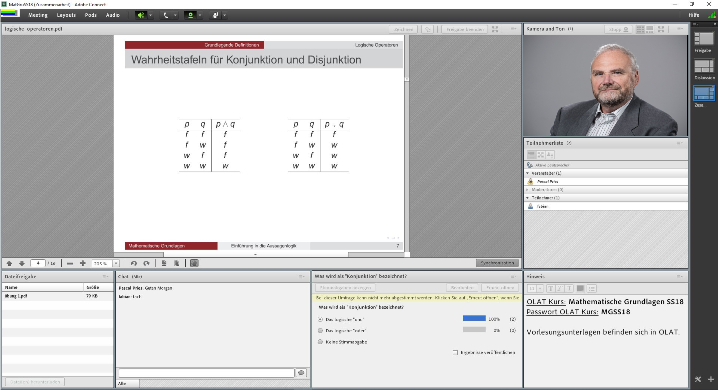
\includegraphics[width=0.98\linewidth]{imagesExample/ConnectOberflaeche1}
%       \caption{Screenshot Connect}
        \label{fig:itasprechstundenlayout}
    \end{figure}

\end{block}

%----------------------------------------------------------------------------------------

\end{column} % End of the first column

\begin{column}{.03\textwidth}\end{column} % Empty spacer column

\begin{column}{.465\textwidth} % The second column


%----------------------------------------------------------------------------------------
%   Digitale Abgabe
%----------------------------------------------------------------------------------------

\begin{block}{Digitale Abgabe}

    \begin{figure}
        \centering
        \includegraphics[width=0.7\linewidth]{imagesExample/digitaleAbgabe2}
        \label{fig:disgitaleabgabe}
    \end{figure}

\end{block}

%----------------------------------------------------------------------------------------
%   GitHub
%----------------------------------------------------------------------------------------

\begin{block}{Werkzeuge aus dem Berufsleben}

    \begin{figure}
        \centering
        
\includegraphics[width=0.8\linewidth]{imagesExample//tools}
        \label{fig:lehrer-octocat}
    \end{figure}

\hspace{0.07\linewidth} Jenkins \hfill GitHub \hspace{0.18\linewidth}

\note{
     \textbf{Warum GitHub?}
\begin{itemize}
    \item Versionsverwaltung erleichtert arbeiten im Team
    \item Wird aktuell viel verwendet / Vorbereitung auf spätere Arbeit
\end{itemize}
\vspace{24px}
\textbf{Wie wird GitHub in der Lehre eingesetzt?}
\begin{itemize}
    \item Arbeitsumgebung / Speicherplatz für Studenten
    \item Verteilung von Aufgaben und Beispielen
    \item Abgabe durch Release-Tags
\end{itemize}
\vspace{24px}
\textbf{Was ist eine GitHub-Organisation?}
\begin{itemize}
    \item  Vorher: Student legt eigenes Repository an $\rightarrow$ Student muss Prof.
    einladen
    \item Erlaubt es dem Prof. Repos für Studenten zu erstellen, auf die er
    dann auch Zugriff hat
    \item beliebig viele private Repos
\end{itemize}
}

\end{block}

%----------------------------------------------------------------------------------------
%   Gamification und neue Lernformen
%----------------------------------------------------------------------------------------

\begin{block}{Gamification}


    \begin{figure}
        \centering
        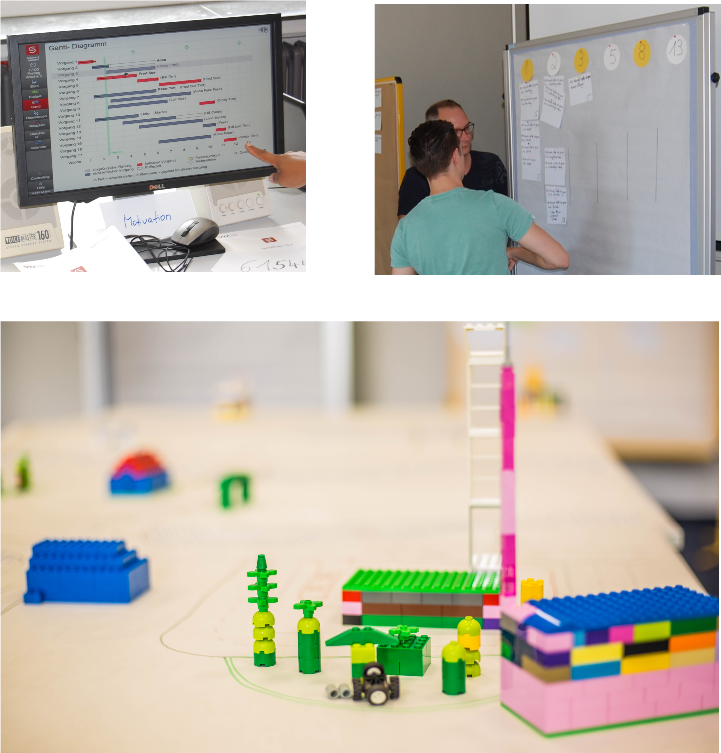
\includegraphics[width=0.76\linewidth]{imagesExample/gamification}
        \label{fig:gamification}
    \end{figure}

\end{block}


% -------------------------------------------
%  Flipped Classroom
% ------------------------------------------
\begin{block}{Flipped Classroom}
    \vspace{40px}
    \begin{figure}
        \centering
        \includegraphics[width=0.8\linewidth]{imagesExample/youtube2}
%       \caption{YouTube}
        \label{fig:youtube2}
    \end{figure}
\end{block}

%----------------------------------------------------------------------------------------

\end{column} % End of the second column

\begin{column}{.015\textwidth}\end{column} % Empty spacer column

\end{columns} % End of all the columns in the poster

\end{frame} % End of the enclosing frame

%\todos

\end{document} 